\chapter{Requirements}
\label{cha:requirements}

This  work  deals with  an  execution  environment  that exploits  virtual
machines,  especially  those  provided  by  the  Xen  hypervisor,  to  run
applications in a  secure environment. Each job that  is submitted to this
execution  environment gets  executed  in its  own  virtual machine,  thus
running in complete independence from other jobs.

In this chapter I am going to describe, how such an environment could look
like and what the main requirements to such a system are.

\begin{figure}[htbp]
  \centering
  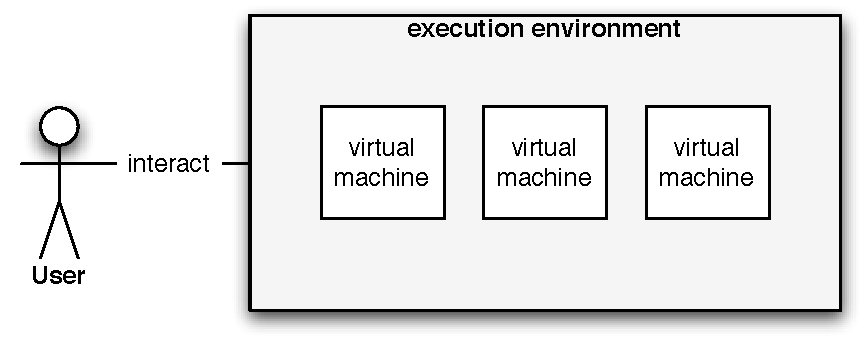
\includegraphics[scale=.7]{concept}
  \caption[Conceptual overview]{A conceptual overview}
  \label{fig:concept}
\end{figure}

The first  glance at  an execution environment  based on  virtual machines
results  in the concept  shown in  Figure~\ref{fig:concept}.  It  shows an
``user'' who is interacting with the execution environment in some way.

\medskip

The next sections describe what  I think, an execution environment must at
least provide to be useful. Furthermore, several use-cases are given, that
show possible usage scenarios of the execution environment.

\section{Execution environment}
\label{sec:req-execution-environment}

What should an execution environment  provide, so that users can work with
it?   I  think the  following  list  gives a  good  idea  about the  basic
requirements any execution environment should at least fulfill:

\begin{itemize}
\item \emph{Submit new tasks} --- i.e.~inform the system about a new task,
  that it should execute.
\item \emph{Query the status of  tasks} --- i.e.~is the task still pending
  and  waiting for  its execution,  currently  running or  did it  already
  finish.
\item \emph{Stop running tasks} --- i.e.~a user must always have the
  possibility to cancel his own tasks.
\item \emph{Security}  --- i.e.~any user of the  execution environment may
  only gain access to his or her own tasks, additionally the tasks have to
  be prohibited from accessing data that belongs to different tasks.
\end{itemize}

Typically, computational tasks  require some input data to  work on. Using
the input data, a task generates output data the user is interested in. To
describe  those  tasks  an  execution environment  demands  the  following
additional requirements:
\begin{itemize}
\item Provision of a way to specify input data for a task
\item Provision of a way to retrieve generated output data from a task
\end{itemize}

Especially in the case of remote  execution, input and output data have to
be  transfered to  and  from  the remote  resource  accordingly. The  next
sections describe each point in more detail.

\subsection{Submission of tasks}
\label{sec:req-task-submission}

In  Grid  environments, for  example,  a user  describes  his  job as  the
application he wants to  execute remotely along with additional parameters
that are to be  passed to the application, input data that  has to be made
available to  the application  prior execution, output  data that  must be
transfered back  to the user  after the application finished,  and various
additional resources that have to be provided at the remote site.

The here proposed execution environment demands a way to describe not only
the tasks, but also  the virtual machine that is going to  be used for the
task. Virtual machines require at least a \emph{kernel} and a full-fledged
operating system installation.

An  upcoming standard  for job  descriptions in  Grid environments  is the
\emph{Job Submission Description Language} --- or \gls{glo:JSDL} for short
(see  Section~\ref{sec:fundamentals:jsdl}  and  \cite{jsdl-spec} for  more
details).  This  specification is  not limited to  be used solely  in Grid
environments;  it  can  be  extended  and adapted  to  fit  any  execution
environment.  The \gls{glo:JSDL} is  an XML-based language that is capable
of describing  a job in all its  details. Due to the  extensibility of the
JSDL, it is rather easy to add descriptions of virtual machines to the job
description.

I  decided to  use this  description language,  so that  the Xen-execution
environment can  easily be integrated  into various middlewares  that also
use  the \gls{glo:JSDL}  to  describe their  jobs.   A common  description
language  of jobs  that are  executed using  the Calana  Grid-scheduler is
still an open topic but the JSDL is a very good candidate.

\subsubsection{Extensions to the \gls{glo:JSDL}}

To be able to create a virtual machine on the remote site, the user has to
specify not only the application she wants  to run but also a kernel and a
file-system   \gls{glo:image}   that    contains   an   operating   system
installation.   The  image  contains  all dependencies  (applications  and
programming libraries etc.) the user's task requires for execution.

The execution environment then takes care of starting up a virtual machine
using the provided  \gls{glo:image} and kernel and is  eventually going to
execute the application within this virtual machine.

The description  of a  virtual machine  cannot be made  by using  just the
elements defined in the \gls{glo:JSDL} specification itself, since one has
to  describe additional locations  for the  \gls{glo:image}, a  kernel and
probably an initial RAM-disk.  Those files are not directly related to the
description  of  a  job  and  therefore  have  no  representation  in  the
specification.

The \texttt{DataStaging} element defined  by the specification seems to be
a good candidate for the descriptionu  of the additional files. But, as it
turns out to be, the \texttt{DataStaging} elements may only refer to files
\textbf{within} the virtual machine. The  files that are used to build the
virtual  machine files  are, on  the other  hand, \textbf{outside}  of the
virtual  machine  (i.e.~outside the  file-system  defined  by the  virtual
machine). That  means that we require  an extension to the  JSDL to define
those files.

\subsection{Query the status of tasks}
\label{sec:status-query}

A user who  has submitted a task to a remote  system for execution, surely
wants to observe the current state of his job. The query for the status of
a job requires the detailed specification of which are the \textbf{allowed
  states} a job can take on and how the \textbf{transitions} between those
states look like.

To provide  the possibility to connect the  Xen-execution environment with
other tools,  a common description for job-states  is required, i.e.~both,
user and  execution environment, must  have the same expectations  on what
the current  state is and  what the next  states could be.

To   the   \emph{Open   Grid   Services   Architecture}   (\gls{glo:OGSA},
\cite{ogsa})  belongs a  working group  that designs  such a  common state
model    for    the   job    execution    in    Grid   or    service-based
environments\footnote{in     \emph{service-based}    environments,    each
  functionality (an \emph{Execution Service}  for instance) is provided by
  a single service (e.g.~a web service).}.  The OGSA is an approach to use
Web service concepts and technologies in a Grid environment.

The just  mentioned working group  defines a special service  that targets
the  execution  of   \emph{activities}  (e.g.~jobs)  ---  the  \emph{Basic
  Execution Service}  (\gls{glo:BES}, \cite{ogsa-bes}).  The specification
defines a basic  and very simple state-model that  describes the execution
of a job (see Section~\ref{sec:fundamentals:bes} and \cite{ogsa-bes} for a
more detailed description).

\subsubsection{Extensions to the BES state-model}

Since the basic \gls{glo:BES} state-model is a very minimal one which does
not satisfy the requirement of data staging, we need to extend it to allow
the  description  of additional  data-transfer  states.  Fortunately,  the
\gls{glo:BES} provides such an extended  model in its specification, it is
shown in  Figure~\ref{fig:bes-extended}. The transfer  of input (stage-in)
and  output  (stage-out)  data  is  part  of  running  the  job,  i.e.~the
additional states are sub-states of the (basic) \texttt{Running} state.

\begin{figure}
  \centering
  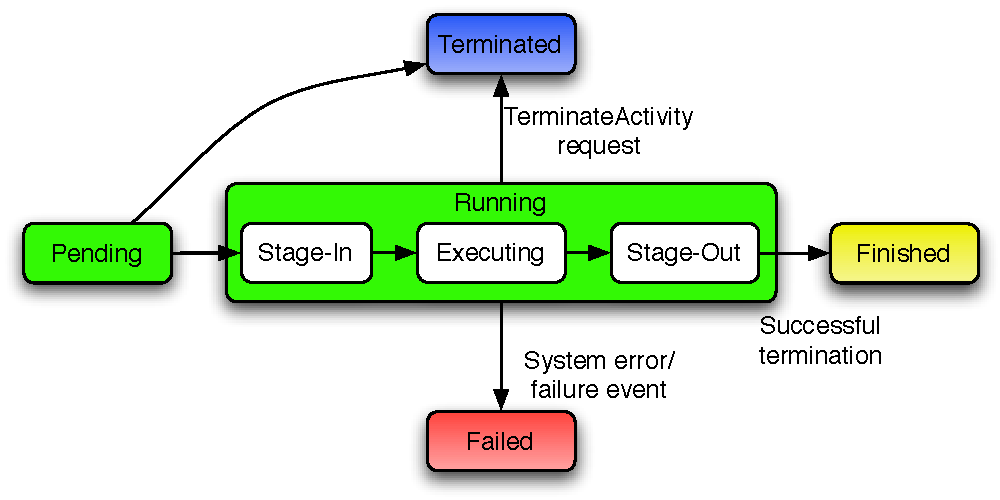
\includegraphics[scale=.75]{bes-staging-job-model}
  \caption[BES State Model Staging Extension]{The basic BES state-model
    extended with sub-states to describe data-transfers.}
  \label{fig:bes-extended}
\end{figure}

The  \texttt{Running}   state  has   been  split  into   three  sub-states
\texttt{Stage-In}, \texttt{Stage-Out} and \texttt{Executing} --- the first
two describe  data-transfer operations and the latter  describes the state
in  which  the task  is  actually  being  executed.  The  \texttt{Running}
sub-state can be seen as the reincarnation of the \texttt{Executing} state
of the  basic model.

Of course,  not all extensions to  the state model are  valid.  An invalid
extension of the specialization, for example, would have been the addition
of a  transition from \texttt{Running:Stage-In}  back to \texttt{Pending}.
This is  because the behavior  of this model,  which an user  observes, is
different from the behavior the basic  model had. An user would not expect
the  current  state of  his  task  to  change from  \texttt{Executing}  to
\texttt{Pending} again.

The \gls{glo:BES} specification, as well as the JSDL specification, define
XML-Schemata, that can be instantiated when needed.  The following example
shows the  usage of  the state description  using XML and  how specialized
sub-states  are represented.  The  main state  is \texttt{Running}  and is
described using the \emph{ActivityStatus} element, any sub-state, that may
currently  be  active,  is   highly  depending  on  the  actual  execution
environment in place and is therefore described using one or more elements
from a different namespace.

\begin{minipage}{0.75\textwidth}
  \begin{lstlisting}[language=XML]
    <bes:ActivityStatus state="Running">
       <n00:Stage-In/>
    </bes:ActivityStatus>
  \end{lstlisting}
\end{minipage}

The example  makes use of  the previously defined  specialized state-model
and  describes an  activity  that is  currently  in the  \texttt{Stage-In}
sub-state of the \texttt{Running} state --- i.e.~the activity is currently
waiting for its  input data to be ready.   The representation allows, that
any client  which is  not aware of  the \texttt{Stage-In}  sub-state, does
only ``see''  that the activity is  in the \texttt{Running}  state. On the
other hand, any client that is aware of this extension, will recognise the
\texttt{Stage-In} element and is able to react accordingly.


\subsection{Stopping tasks}
\label{sec:stopping-task}

Well, as  you can see in  Figure~\ref{fig:bes-extended}, each non-terminal
state  of  the  model provides  a  transition  to  the state  final  state
\texttt{Terminated}. This behavior does directly resemble the requirements
for \emph{stopping a  task} on behalf of an user  request.  An user of
any execution environment should be able to stop the execution of her task
at any time regardless of the task's current state --- final states are an
exception, of course.

In  case of  this work,  stopping  a task  may involve  shutting down  the
virtual machine, terminating currently active data transfers and releasing
acquired resources.

\subsection{Security issues}

There  are  several  issues  related  to  security  when  implementing  an
execution  environment, especially  when the  execution takes  place  on a
remote machine. The most crucial  issue is the \emph{limitation of access}
to the system,  i.e.~how are the users identified that  are allowed to use
the system.   Another issue  is \emph{privacy of  communication}, i.e.~can
the  communication  between  an  user  and the  execution  environment  be
overheard  by  some  (potentially  malicious)  entity  (another  user  for
instance).  Furthermore  the tasks have  to be executed in  a \emph{secure
  and independent environment}.

A typical  approach in  Grid middlewares such  as Globus  \cite{globus} or
Unicore    \cite{unicore}   is    to   use    cryptographic   certificates
(e.g.~\gls{glo:X509}  certificiates) for authentication  and authorization
purposes, the \gls{glo:XenBEE} should follow the same principles.

\subsubsection{Authentication and Authorization}

Authentication  and  authorization are  to  be  realized using  public-key
certificates  following  the   \gls{glo:X509}  specification.   A  special
certificate authority  can be  used to issue  certificates to  those users
that want to access the \gls{glo:XenBEE}.

The  use   of  certificates  issued   by  a  trusted  authority   forms  a
\gls{glo:PKI}   and   therefore    provides   authentication   among   the
components. A user  who wants to gain access  to the execution environment
is required to  acquire a certificate signed by  that authority first. The
same holds for the other way around, a user can verify the authenticity of
a server using the server's certificate.

Authorization  can   be  implemented  by  further   limiting  the  allowed
certificates.   The server  could,  for instance,  consult  a database  of
certificates. This database would contain each certificate that is allowed
to  access the execution  environment. That  means an  user can  only gain
access to the  system, if his certificate has been  issued by an authority
the server trusts  \textbf{and} his certificate is listed  in the server's
database.

Since the server does know the user  and is able to identify him, any task
the user submits  can be annotated with a token  representing the owner of
the  task.  A  request to  that task  could then  be checked  against this
annotation and eventually be allowed or denied.

\subsubsection{Privacy}

Since   the  mentioned   certificates  contain   a   public-key,  standard
cryptographic  algorithms can  be used  to implement  secure communication
between user and server.  Section~\ref{sec:secure-communication} considers
public-key  cryptosystems  and  communication  security  on  the  base  of
\emph{Message Layer Security}.

\subsubsection{Task execution security}

The main topic  of this work is, that tasks are  separated from each other
by the use  of virtual machines.  Therefore execution  security as such is
maintained but the same must hold  for data transfers for example. An user
must not be allowed to access or modify the files of any other user.

\section{A more concrete concept}

The previous  sections dealt with a  rather abstract view  on the proposed
execution  environment,  this section  however  outlines  a slightly  more
concrete  concept  for  the  execution  environment  and  its  components.

Handling of requests, that the users make to the execution environment and
controlling the  virtual machines, requires an  additional component. This
component will be called  \emph{Xen-based Execution Daemon} or \emph{xbed}
for short. If an user wants to interact with the execution environment, he
does  so  by  communicating  directly  with the  managing  component  (see
Figure~\ref{fig:concrete-concept}).

\begin{figure}[htbp]
  \centering
  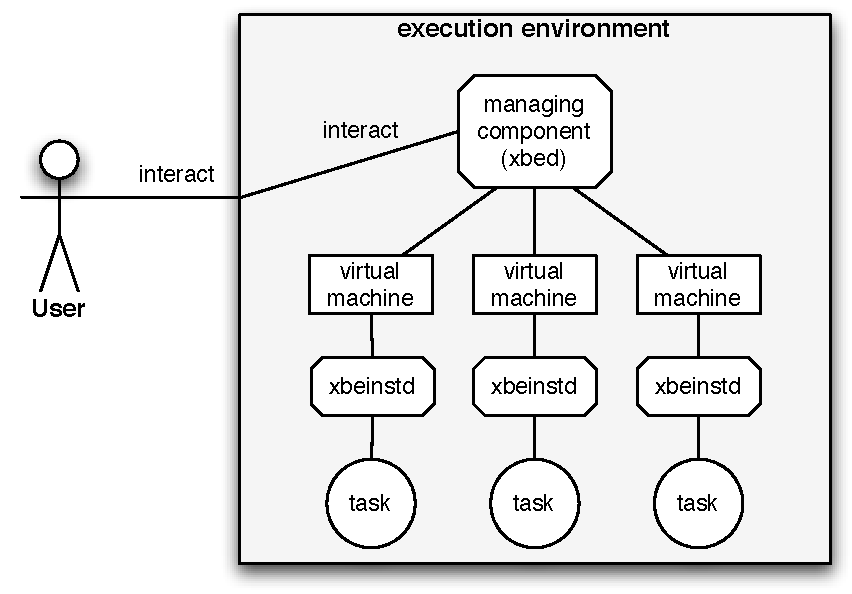
\includegraphics[scale=.7]{concrete-concept}
  \caption[A more concrete concept]{The  evolved concept, using a managing
    component (\emph{xbed}) to control the virtual machines.  Each virtual
    machine  is  dedicated  to  a  single  task  submitted  by  some  user
    (controlled  through the  \emph{xbeinstd} component).   Users  do only
    interact with the managing component.}
  \label{fig:concrete-concept}
\end{figure}

Another component which  will be required to control  the actual execution
of a task  within a virtual machine will  be the \emph{Xen-based Execution
  Instance Daemon} or \emph{xbeinstd} for short. There are several reasons
why this  dedicated component  is required to  be running in  each virtual
machine. The  most important one is,  that the same  virtual machine image
could  be used  for more  than just  one application.   Another  reason is
simply flexibility,  the \gls{glo:JSDL} allows an user  to exactly specify
how and which application shall be run and this component adheres to that.

\bigskip

Basically  this concept  defines a  client-server architecture,  where the
client is represented  by the user (or some mediator  such as a web-portal
or a  command-line client) and the  server is represented  by the managing
component.

The interaction between the users and the execution environment requires a
communication   layer   over   which    the   requests   are   made.    In
Section~\ref{sec:fundamentals:mom} I have already introduced \emph{Message
  Oriented  Middlewares} and  how  message-queue servers  can  be used  to
provide logical  connections between the  involved distributed components.
Using the  same concept in this  execution environment makes  sense due to
the following reasons:

\begin{itemize}
\item  There could be  more than  one server  providing such  an execution
  environment.   Message-queue \emph{topics}\footnote{A \emph{topic}  is a
    special queue to  which arbitrary many consumers can  subscribe.  If a
    message gets sent to this  queue, all consumers (rather than just one)
    receive  this message.}  can  be used  to handle  any number  of those
  servers uniformly. The clients send  their requests to a single queue on
  the  \gls{glo:MQS} and  the \gls{glo:MQS}  multiplexes it  to  all known
  servers.
\item The server could be in  need of sending messages to clients that are
  not connected anymore. Think of a notification that could be sent when a
  task finished its execution.
\item The use of a MQS renders  it possible that the server can be located
  behind a very restrictive firewall or even a \gls{glo:NAT}-gateway.
\item The  Calana scheduler  uses also a  \gls{glo:MQS} to  connect users,
  broker and agents.
\item  There is  no visible  difference for  a client,  whether it  uses a
  direct connection or a connection through a \gls{glo:MQS}.
\end{itemize}

The  network  layers  that  are  involved when  using  a  message-oriented
communication    with    a    message-queue    server   are    shown    in
Figure~\ref{fig:mqs-layers}.

\begin{figure}[htbp]
  \centering
  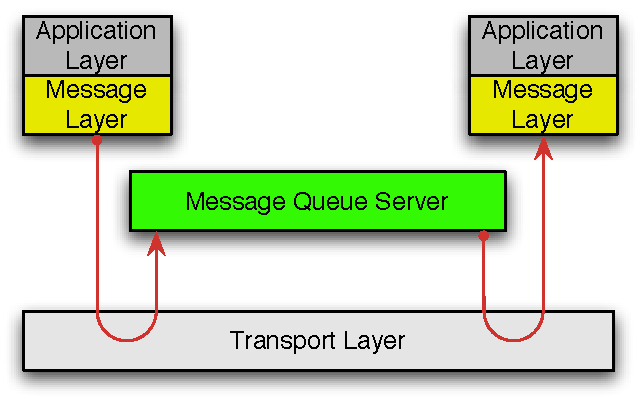
\includegraphics[scale=0.7]{mqs-layers}
  \caption[Message Layers]{Message-oriented communication layers.}
  \label{fig:mqs-layers}
\end{figure}


\section{Use cases}
\label{sec:use-cases}

This section describes possible use cases for the \gls{glo:XenBEE}. I have
already shortly described, what the  basic requirements to this system are
and now  I am  going to show  you some  use cases and  which parts  of the
architecture are involved in each of them.

The ``big picture'' is shown in Figure~\ref{fig:system-usecases}, it shows
a compendium  of several possible  use cases from  a very high  level. The
involved    actors    are     the    \emph{user},    the    \emph{managing
  component}\footnote{denoted as \emph{xbed} --- the ``Xen-based Execution
  Daemon''}     mentioned      earlier     and     a      new     managing
component\footnote{denoted   as   \emph{xbeinstd}   ---  the   ``Xen-based
  Execution Instance Daemon''} which  is running on and solely responsible
for a single virtual machine.

\begin{figure}[htbp]
  \centering
  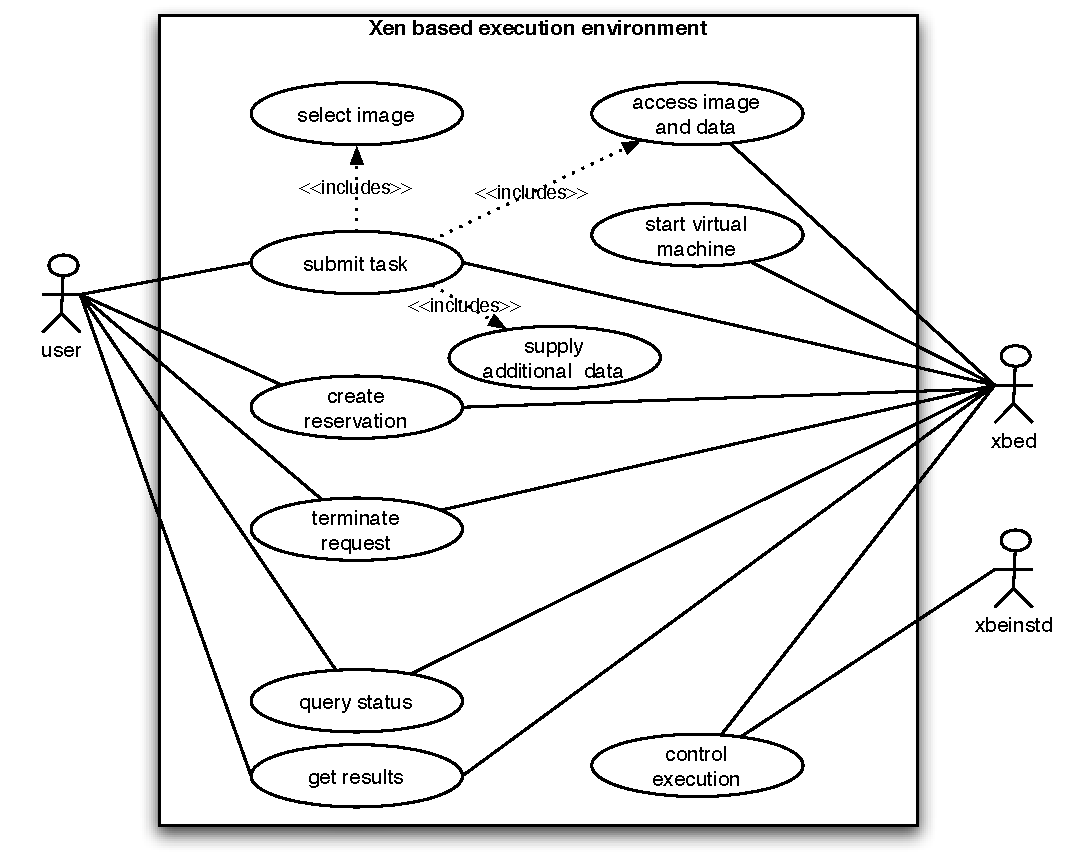
\includegraphics[scale=0.7]{system-usecase}
  \caption[Use case  overview]{An overview  of several possible  use cases
    and the involved actors.}
  \label{fig:system-usecases}
\end{figure}

\subsection{Task submission}
\label{sec:uc-task-submission}

The very  first use case is  the submission of a  \emph{simple} task. With
\emph{simple} I mean, that the  task does not require any additional data,
it just  requires a previously prepared \gls{glo:image}  that contains the
application and the \emph{xbeinstd}.

On  server-side, the  \emph{xbed}  will associate  the  submission with  a
previously acquired  reservation ---  i.e.~the user creates  a reservation
first  which results in  some kind  of handle  (a unique  identifier which
refers to the  reservation) and then the user submits  his task using that
reservation.

\begin{figure}[htbp]
  \centering
  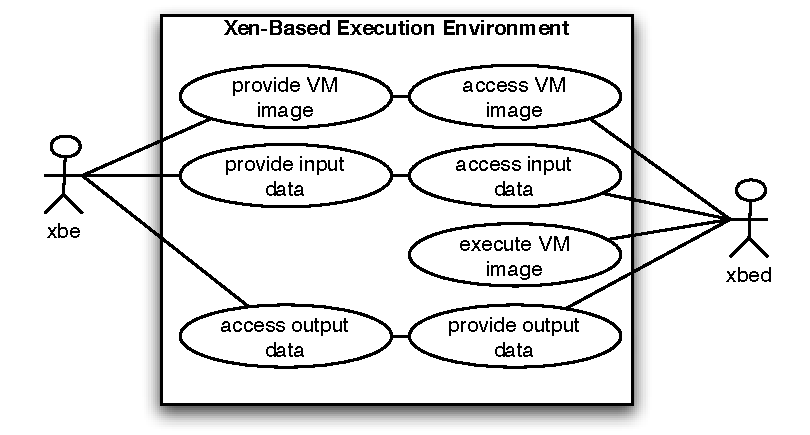
\includegraphics[scale=.75]{uc-submit-task}
  \caption[UC Task submission]{Actors involved  in the task submission use
    case.}
  \label{fig:uc-submit-task}
\end{figure}

\paragraph{Selecting an image}
In  Figure~\ref{fig:uc-submit-task} the  required steps  for  submitting a
task are  shown. The  submission of  a task includes  the selection  of an
image  that  contains  the  application  the user  wants  to  execute.   A
sophisticated process of image-selection  can be rather complicated, since
it involves matching of available images against a description provided by
the user. Such  selection mechanisms are out of the  scope of this thesis,
but  in  a  later  use  case,  server-side  \emph{caching  of  data}  (see
Section~\ref{sec:uc-data-caching}),  a  simple way  of  selection will  be
described.

\paragraph{Accessing the image}
After the user submitted a  task, the \emph{xbed} has to \emph{access} the
specified image,  i.e.~the \emph{xbed} will initiate the  retrieval of the
image.   The  location  of  the  image  can for  example  be  given  as  a
\gls{glo:URI}  to   provide  an  uniform  and   extensible  mechanism  for
describing data locations.

If errors occur  during the image retrieval, the  \emph{xbed} has to abort
the task execution and must inform the user about the failure.

\subsection{Data staging}
\label{sec:uc-data-staging}

This  use case  is an  enhancements  over the  previous one,  it not  only
involves the  submission of an image,  but also the  specification of data
that  must  be  available  prior  executing  the task  and  that  must  be
transfered back to user after the task has finished.

\begin{figure}[htbp]
  \centering
  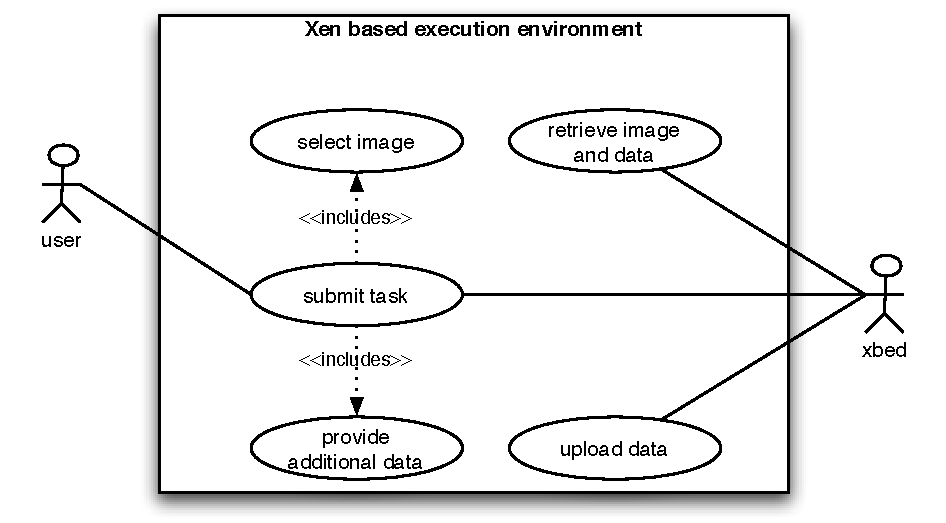
\includegraphics[scale=.75]{uc-data-staging}
  \caption[UC  Data  Staging]{A user  submitting  a  task with  additional
    data.}
  \label{fig:uc-data-staging}
\end{figure}

Again,  the JSDL comes  into play  here, because  it already  supports the
description of staging operations. The \emph{xbed} has now to retrieve not
only  the image  file, but  also  all the  additional files  the user  has
specified to be staged in.

After the job  has finished its execution, the  \emph{xbed} is responsible
for staging  out generated  files. Therefore the  user must  specify which
files that are and to which locations they have to be uploaded. Source and
destination locations of files can again be specified as \gls{glo:URI}s.

\subsection{On-demand VM-deployment}
\label{sec:uc-on-demand-vm-deployment}

Well, this use  case can be seen  as a variant of the  task submission use
case. The purpose of this use case is the creation of a virtual machine on
user request without executing any task.

The resulting virtual  machine could be accessed by  the user through some
remote mechanism such as \gls{glo:SSH} \cite{openssh}.  With \gls{glo:SSH}
the  user gains  full control  over his  created virtual  machine  and can
install, setup and run any application he likes.

The login to  the \gls{glo:VM} can be provided  by using SSH's public-keys
that  are either  previously installed  into the  image or  uploaded later
using  the standard  stage-in  mechanisms provided  by the  \gls{glo:JSDL}
(please consult the documentation on \gls{glo:SSH} for further information
about authorization with public-keys).


\subsection{Caching of data}
\label{sec:uc-data-caching}

Imagine a user,  who wants to execute the  same application several times.
That would mean he has to submit the same image over and over again, which
imposes a heavy load on the network connecting user and provider (i.e. the
host on which the \emph{xbed} runs). It would be wise to provide a caching
mechanism, that  allows the  user to store  his image on  server-side. The
caching efficiently  reduces network load and  decreases overall execution
time \cite{locality-principle}.

\begin{figure}[h]
  \centering
  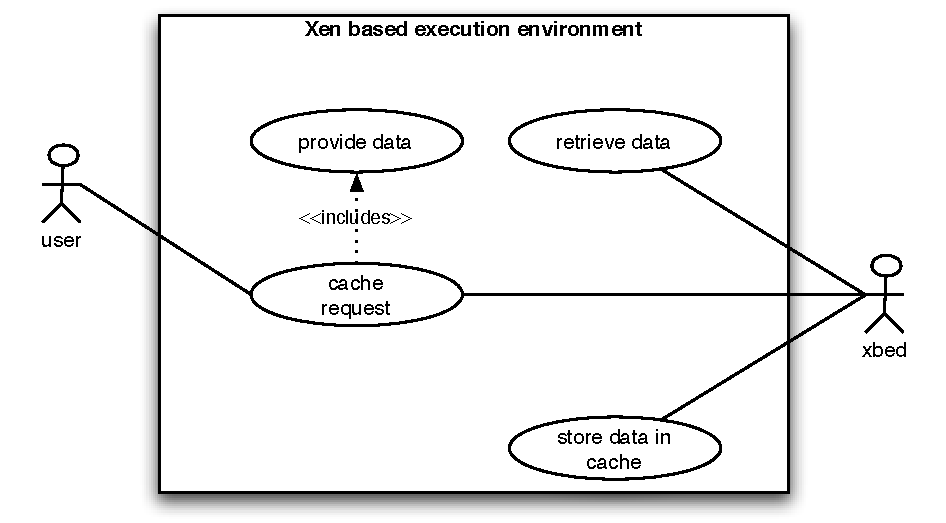
\includegraphics[scale=.75]{uc-data-caching}
  \caption[UC  Data  Caching]{A user  who  is  requesting  the caching  of
    (arbitrary) data.}
  \label{fig:uc-data-caching}
\end{figure}

In  Figure~\ref{fig:uc-data-caching} the required  steps for  caching some
data are  shown. The user  makes his request  for caching the data  to the
\emph{xbed}, which in turn retrieves the data and stores it in a cache. To
make  the ``discovery''  of cached  data easier  for the  users,  the user
should be required to give some descriptive information for the data he is
going to  cache. As the return of  the request, the user  should receive a
unique identifier or an \gls{glo:URI} for the created entry in the cache.

The details  of how  exactly the caching  works are  highly implementation
specific, the most important point is  how the cached data can be referred
to by users of the system at a later point in time.

\paragraph{Referencing cached  data}

Cached data must be referable by the user for subsequent task submissions.
Since the submission of tasks uses \gls{glo:URI}s to indicate the location
of a  file, an obvious  way is  to use a  \gls{glo:URI} here as  well. The
caching of some data should  therefore result in a \gls{glo:URI}, that the
user can use in his job and staging descriptions.

\begin{figure}[h]
  \centering
  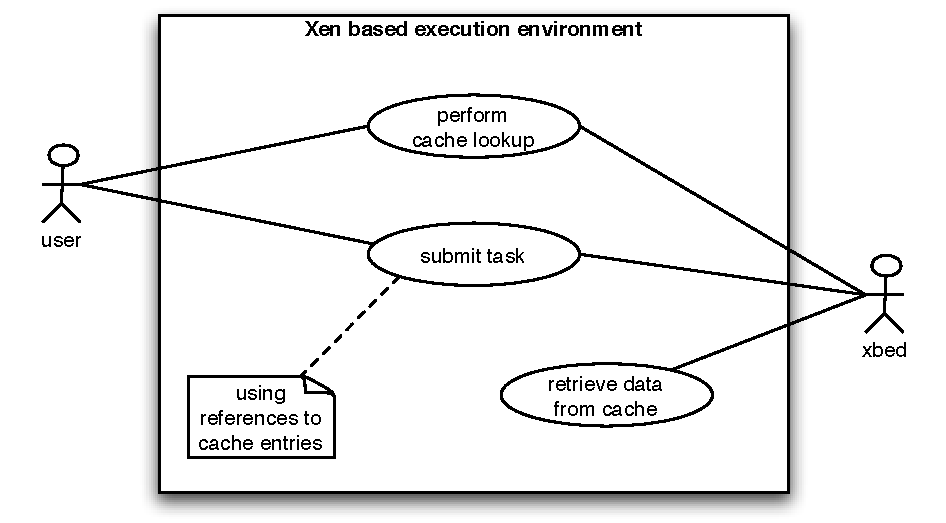
\includegraphics[scale=.75]{uc-cache-lookup}
  \caption[UC  Cache Lookup]{A user  who  is using cached entries within
    his task submission.}
  \label{fig:uc-cache-lookup}
\end{figure}

Additionally, a really  nice thing to have in this  situation is some kind
of a lookup mechanism for cached  entries --- i.e.~a user does not need to
remember all the  \gls{glo:URI}s his entries have, but can  use a query to
the    system   and   thus    figure   out,    which   cache    entry   to
use. Figure~\ref{fig:uc-cache-lookup} shows you  how a user looks up cache
entries and uses them in a subsequent task submission.

\subsection{Terminating a task}
\label{sec:uc-terminate-task}

As   you   could   see   in   the   \gls{glo:BES}   job   state-model   in
Figure~\ref{fig:bes-extended},  the  user  must  have the  possibility  to
terminate his  submitted task at any  time and no matter  what the current
state of the task is.

\begin{figure}[h!]
  \centering
  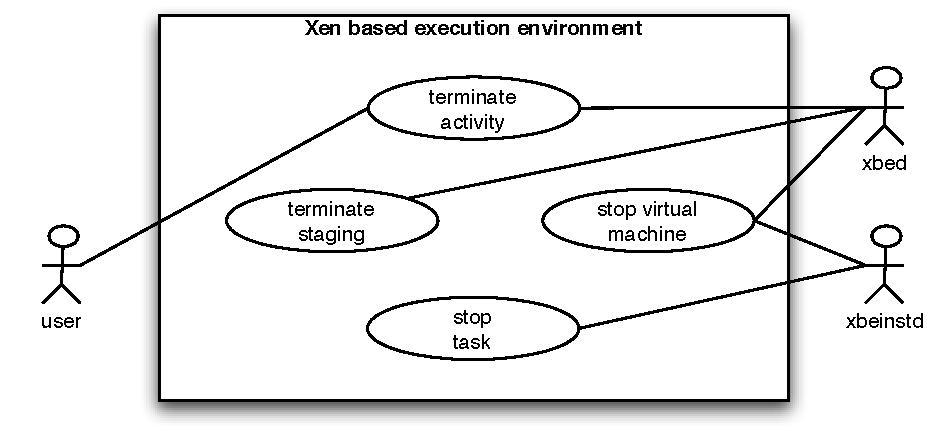
\includegraphics[scale=.75]{uc-terminate-task}
  \caption[UC Terminate Task]{A user  who is requesting the termination of
    his  submitted task  and possible  use cases  that may  then  arise on
    server-side.}
  \label{fig:uc-terminate-task}
\end{figure}

The termination request  for a task can be received in  any state and that
may require  additional actions to be  taken in the  \emph{xbed}.  If, for
instance,  a virtual  machine has  already been  created and  is currently
executing the user's task, the application and the virtual machine have to
be terminated, too.  The same  holds for staging activities, that could be
currently active, they  have to be terminated cleanly  as well.  These use
cases are  shown in  Figure~\ref{fig:uc-terminate-task}. As you  can seen,
the \emph{xbeinstd} may be involved again, since the actual execution of a
task falls within his responsibility.

\subsection{Providing encrypted data}
\label{sec:uc-ecrypted-data}

Since all  data is referred to  by \gls{glo:URI}s, that  may be accessible
not  only  from  the  \emph{xbed}  itself, but  also  from  other  sources
(i.e.~probably unknown and  hostile ones), it is desirable  to store those
files encrypted. Of  course, if a user stores  an encrypted image-file and
wants  the \emph{xbed} to  use it  for execution,  the image-file  must be
decrypted on server-side prior booting a virtual machine with it.

\begin{figure}[h]
  \centering
  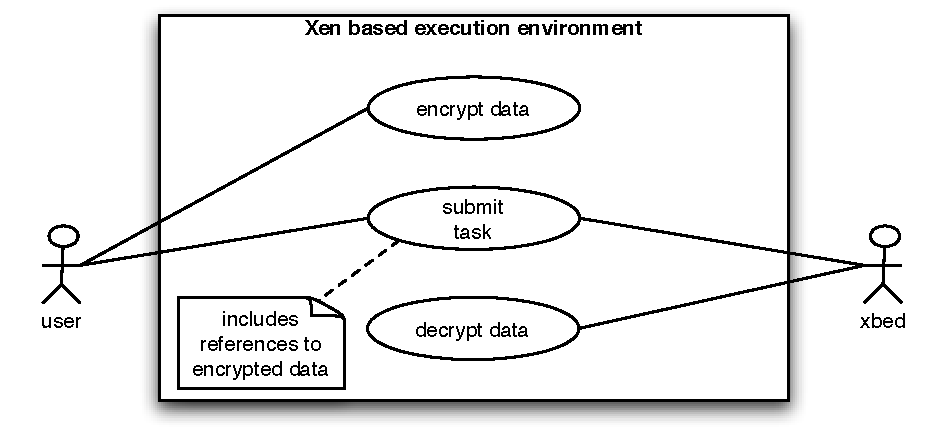
\includegraphics[scale=.75]{uc-encrypted-data}
  \caption[UC  Encrypted  Data]{Submission   of  encrypted  data  and  its
    decryption prior execution by the \emph{xbed}.}
  \label{fig:uc-encrypt-data}
\end{figure}

A user  can apply any kind of  encryption to the data.  The \emph{xbed} in
turn must provide a way for the  user to specify how and probably when the
data  should  be decrypted.   For  instance,  the  user could  provide  an
encrypted  virtual machine  image and  the \emph{xbed}  has to  decrypt it
prior  starting the  virtual machine.   But  the user  could also  provide
encrypted  input data for  the application  he wants  to execute,  then it
would be up  to the user whether the data is  decrypted by the \emph{xbed}
or by the application itself.

\subsection{Support for Calana}
\label{sec:calana-support}

To  support  Calana, the  \gls{glo:XenBEE}  must  provide some  additional
functionality. One of these functionalities is a mechanism to \emph{make},
\emph{cancel}   and   \emph{confirm}   reservations.   To   reflect   that
requirement in the  way jobs are represented, we  discussed about a common
state-model  for  the jobs  and  came to  the  consensus  of adopting  the
\gls{glo:BES}         model        to        our         needs        (see
Figure~\ref{fig:bes-calana-job-model}).

\begin{figure}[h]
  \centering
  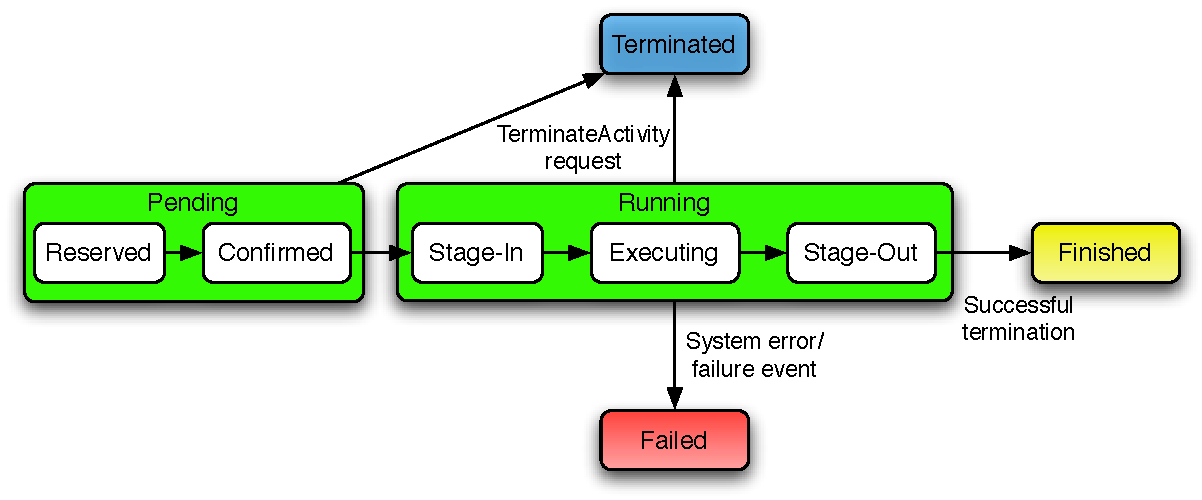
\includegraphics[scale=.55]{bes-calana-job-model}
  \caption[Calana Job Model]{The common job model proposed by the Calana
    Grid scheduler.}
  \label{fig:bes-calana-job-model}
\end{figure}

The common  job model includes extensions to  describe staging operations,
as well as an extension to support reservations. When an activity is still
pending it  can be  either \texttt{Reserved} or  \texttt{Confirmed}. These
states reflect the state a Calana-agent  is in when reacting on an auction
that  has  been opened  by  some  broker. While  an  auction  is still  in
progress, the  reservation is \emph{pending}  until it is canceled  due to
the loss of  that auction or it is won  and eventually \emph{confirmed}.

% The implementation of  Calana, which is to the time  of this writing still
% in development,  uses also message  queues to implement  the communication
% between consumers, brokers and agents.

\bigskip

The picture  in Figure~\ref{fig:calana-xenbee} describes how  a user would
interact  with  a  system,  that   uses  Calana  for  scheduling  and  the
\gls{glo:XenBEE} as  its execution environment. The user  first requests a
resource from  the broker, who in turn  will open up an  auction among the
agents.  One of those agents are  shown in the figure. The agent creates a
reservation on the \emph{xbed} to which he is connected.

\begin{figure}[htbp]
  \centering
  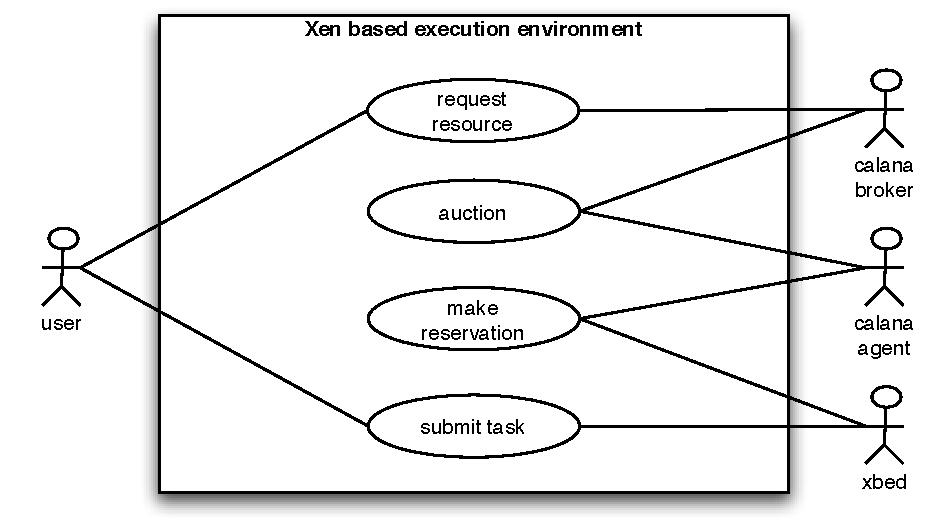
\includegraphics[scale=0.7]{uc-calana-xenbee}
  \caption[Calana and  XenBEE]{The actors and use cases  that are involved
    when a Calana agent uses the \gls{glo:XenBEE} as its resource.}
  \label{fig:calana-xenbee}
\end{figure}

The user is  eventually presented a unique identifier  for his reservation
which he  can use to submit  his task to the  \emph{xbed}. The \emph{xbed}
should  then check the  validity of  the reservation  a user  provides and
probably deny the job submission. Again, the \gls{glo:JSDL} document, used
to  describe  the  job,  can  provide all  required  information  for  the
reservation.   In this  case, the  specification does  already  suggest an
extension to the \texttt{Resources} element,  that can be used to describe
\emph{tickets}. A ticket can be  seen as a handle identifying a previously
made reservation.

%%% Local Variables: 
%%% mode: latex
%%% TeX-master: "main.tex"
%%% End: 
